\documentclass[11pt,a4paper]{article}
\usepackage[margin=0.8in]{geometry}
\usepackage{fontspec,unicode-math,booktabs,graphicx,hyperref}
\setmainfont{STIXGeneral}\setmathfont{STIX Two Math}
\title{Chamber orbits and regular covers:\\complete manuscript costs}
\author{Human Compression project}\date{}
\begin{document}\maketitle
The sources are Zhang and Leemans, \emph{Testing chirality on hypertopes}
(L008, arXiv 2511.14562v1, November 2025), and Cunningham,
\emph{Chiral polytopes whose smallest regular cover is a polytope} (N016, the eight-page
25 July 2023 author edition). N016's publisher PDF was not available.
We compare two complete source manuscripts with the complete common
paper and both applications. The 27 detailed records describe these two
principal contracts; they are not 27 manuscripts.

\paragraph{Whole topic and individual applications.}
The primary unit is calibrated NFC characters without whitespace. Exact
running headers and page numbers are removed; titles, abstracts, references,
source code and extractable tables remain included.
\begin{center}\begin{tabular}{lrr}\toprule
Complete document & Pages & Characters\\\midrule
Source L008 & 10 & 21784\\
Source N016 & 8 & 14018\\
Common theory $U_H$ & 6 & 15199\\
Chirality application H1 & 3 & 7571\\
Regular-cover application H2 & 6 & 13683\\
Whole two-program appendix & 3 & 7677\\\bottomrule
\end{tabular}\end{center}
The whole-topic written comparison is
\[
 R_{\mathrm{written}}=\frac{21784+14018}{15199+7571+13683}
 =\frac{35802}{36453}=0.982.
\]
The complete written replacement is slightly longer in this unit. Once the
\emph{whole common paper and both complete programs} have been acquired,
the conditional comparisons are
\[
 r_1\mid(U_H,P_H)=\frac{21784}{7571}=2.877,\qquad
 r_2\mid(U_H,P_H)=\frac{14018}{13683}=1.024.
\]
Both applications are shorter than their matched sources in this unit, but
these conditional factors do not pay for the common acquisition again.
Every topic pays for its own whole common theory even when proofs overlap.

\paragraph{Complete programs and the limits of the comparison.}
The GAP program is a premise for the six finite groups and their maps;
the Python program validates separately proved action formulas. Both files
are charged in full. Including their printed appendix gives
$35802/(36453+7677)=0.811$. The raw files instead cost 6401
(3528 required; 2873 diagnostic), giving
$35802/42854=0.835$. These representations are alternatives,
never added together. Three operational drivers cost 13158 separately;
three Lean files cost 8605 separately and contain fourteen scoped
component declarations, seven new and seven reused. This is not a complete
Lean verification of either application.
\newpage
\begin{center}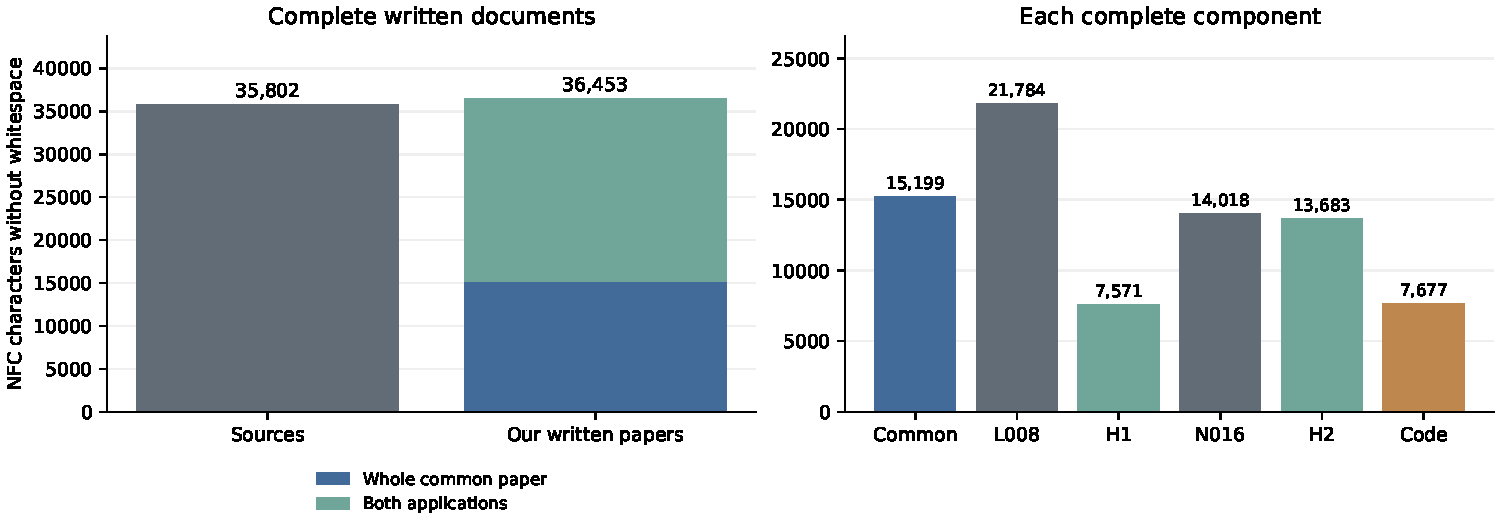
\includegraphics[width=\textwidth]{complete_costs.pdf}\end{center}
The left panel pays for the whole common paper and both applications.
The right panel shows each complete document separately, including code.
These text lengths do not establish minimum proof complexity or a recurring
sawtooth pattern.

\paragraph{Sensitivity to the measurement convention.}
For calibrated selected text with NFC normalization:
\begin{center}\begin{tabular}{lrrr}\toprule
Unit & Whole written & L008/H1 & N016/H2\\\midrule
Whitespace words & 1.022 & 2.704 & 1.182 \\
Alphanumeric units & 1.070 & 3.004 & 1.149 \\
Nonspace characters & 0.982 & 2.877 & 1.024 \\
Characters, collapsed spaces & 0.989 & 2.846 & 1.051 \\
UTF-8 bytes, collapsed spaces & 0.940 & 2.617 & 1.023 \\
\bottomrule\end{tabular}\end{center}
All five units are retained under NFC and NFKC for raw untrimmed, raw
selected and calibrated selected text. The thirty coordinates provide
150 exact fractions: ninety whole-topic and sixty conditional. Small
factors near one should be read with this unit sensitivity, not as a claim
that every reasonable encoding gives the same conclusion.

\paragraph{What the source comparison covers.}
L008's principal finite chirality criterion is recovered. For infinite groups,
its numerical cardinality condition is replaced by the exact two-coset
condition. The printed source software and other ancillary claims are
outside the replacement contract, although their text remains in the
complete-source numerator. N016's proved conclusions are recovered for
its fixed author edition, including all five specified atomic families and
the six-group example. The correction excluding \emph{nonidentity} powers
and the retained Cunningham--Pellicer family classification remain explicit.

Standard geometric correspondences, the Schulte--Weiss section theorem,
the square-tessellation identification and that classification are retained
at their points of use. Their complete proof costs remain unknown, as do
unavailable historical software, graphics and formula layout. The later
unrestricted-cover answer and finite-rank extensions are separate results,
not unpriced premises here; all-rank finite minimal-cover multiplicity
remains unresolved. This measurement adds no source or question credit.

\paragraph{Input and review boundary.}
The independently accepted input audit covers all 36 pages, 180 PDF and
80 raw-file measurements, 34 actual font dictionaries and 893 used glyph
classes. It preserves 36 visible delimiter pieces and two bitmap bullets
among 217 occurrence repairs. Raw alternatives remain available. Extraction
uses pypdf 6.13.0 and fontTools 4.63.0; it does not measure complete visual
information. This numerical edition still requires distinct independent
arithmetic and reader review before publication.
\end{document}
